\documentclass[tikz,border=10pt]{standalone}
\usepackage{tikz}
\usetikzlibrary{positioning}
\usetikzlibrary {arrows.meta}
\usetikzlibrary{calc}
\usetikzlibrary { decorations.pathmorphing, 
decorations.pathreplacing, decorations.shapes,}
\usepackage{unicode-math}
\setmathfont{XITS Math}
\begin{document}

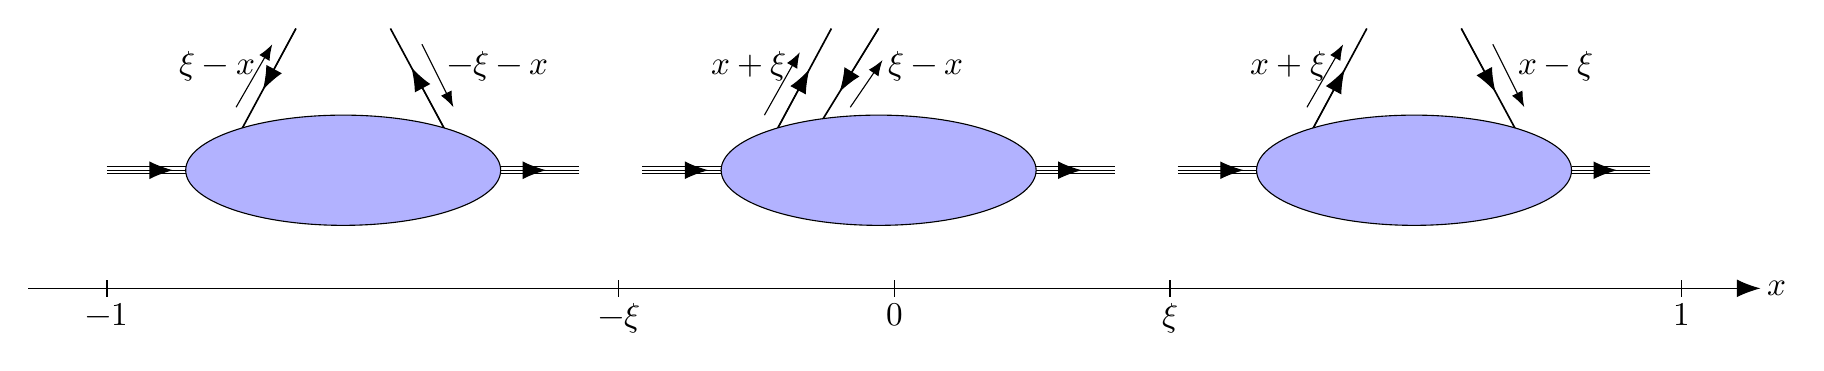
\begin{tikzpicture}[font=\large]
    \begin{scope}
        %%start----subpicture 代码
        \coordinate (a0) at (0,0){};
        \node[above right =-1.5 and -0.2 of a0](Flabel){};% 图的 label
        %% 入射和出射核子
        \coordinate[above right =0 and -1.6 of a0] (a1){};
        \coordinate[above right =0 and -3.0 of a0] (b1){};
        \node[above right =0 and -3.2 of a0,align=right] (b1l){}; % 核子标记
        \coordinate[above right =0 and 2.0 of a0] (a2){};
        \coordinate[above right =0 and 3.0 of a0] (b2){};
        \node[above right =0 and 3.0 of a0,align=left] (b2l){};
        % 核子连线
        \draw[double,double distance=2pt] (b1)--(a1);
        \draw[double,double distance=2pt,-{Latex[length=3mm]} ] (b1)--($(b1)!.6!(a1)$);
        \draw (b1)--(a1);
        \draw[double,double distance=2pt] (b2)--(a2);
        \draw[double,double distance=2pt,-{Latex[length=3mm]} ] (a2)--($(a2)!.58!(b2)$);
        \draw (b2)--(a2);
        %入射和出射部分子
        \coordinate[above right =0.5   and 1.3 of a0] (a3){};
        \coordinate[above right =1.8   and 0.6 of a0] (b3){};
        \draw[semithick] (b3)--(a3);
        \draw[-{Latex[length=3mm]} ] (a3)--($(a3)!.62!(b3)$);
        % 部分子标记
        \node[above right =1.0   and 1.2 of a0,align=left] (b3l){$-\xi-x$};
        % 动量标记
        \coordinate[above right =0.8  and 1.4 of a0] (a3m){};
        \coordinate[above right =1.6  and 1.0 of a0] (b3m){};
        \draw[-{Latex[length=2mm]} ] (b3m)--(a3m); % b3m上端
        %%
        \coordinate[above right =1.8 and -0.6 of a0] (b4){};
        \coordinate[above right =0.5 and -1.3 of a0] (a4){};
        \draw[semithick] (b4)--(a4);
        \draw[-{Latex[length=3mm]} ] (b4)--($(b4)!.6!(a4)$);
        \node[above right =1.0   and -2.2 of a0,align=right] (b4l){$\xi-x$};
        %%部分子连线
        \coordinate[above right =1.6 and -0.9 of a0] (b4m){};
        \coordinate[above right =0.8 and -1.36 of a0] (a4m){};
        \draw[-{Latex[length=2mm]} ] (a4m)--(b4m); % a4m 下端
        % 画椭圆 blob
        \filldraw[fill=blue!30,draw=black] (a0) ellipse [x radius=2cm,y radius=.7cm,anchor=center];
        %%end-----subpicture 代码
    \end{scope}

    %%+++++++++++++++++++++++++ 图2
    \begin{scope}[xshift=6.8cm]
        %%-----subpicture 代码
        \coordinate (a0) at (0,0){};
        \node[above right =-1.5 and -0.2 of a0](Flabel){};% 图的 label
        %% 入射和出射核子
        \coordinate[above right =-0 and -1.6 of a0] (a1){};
        \coordinate[above right =0 and -3.0 of a0] (b1){};
        \node[above right =0 and -3.0 of a0,align=right] (b1l){}; % 核子标记
        \coordinate[above right =-0 and 2.0 of a0] (a2){};
        \coordinate[above right =0 and 3.0 of a0] (b2){};
        \node[above right =0 and 3.0 of a0,align=left] (b2l){};
        % 核子连线
        \draw[double,double distance=2pt] (b1)--(a1);
        \draw[double,double distance=2pt,-{Latex[length=3mm]} ] (b1)--($(b1)!.6!(a1)$);
        \draw (b1)--(a1);
        \draw[double,double distance=2pt] (b2)--(a2);
        \draw[double,double distance=2pt,-{Latex[length=3mm]} ] (a2)--($(a2)!.58!(b2)$);
        \draw (b2)--(a2);
        %入射和出射部分子
        \coordinate[above right =0.5 and -0.8 of a0] (a3){};
        \coordinate[above right =1.8 and 0.0 of a0] (b3){};
        \draw[semithick] (b3)--(a3);
        % 部分子标记
        \node[above right =1.0   and 0.0 of a0,align=left] (b3l){$\xi-x$};
        % 动量标记
        \coordinate[above right =1.4 and 0.05 of a0] (b3m){};
        \coordinate[above right =0.8 and -0.36 of a0] (a3m){};
        \draw[-{Latex[length=2mm]} ] (a3m)--(b3m); % 下端->上端
        %%
        \coordinate[above right =1.8 and -0.6 of a0] (b4){};
        \coordinate[above right =0.5 and -1.3 of a0] (a4){};
        \draw[semithick] (b4)--(a4);
        \coordinate[above right =1.5 and -1 of a0] (b4m){};
        \coordinate[above right =0.7 and -1.45 of a0] (a4m){};
        \draw[-{Latex[length=2mm]} ] (a4m)--(b4m); % 下端->上端
        %%部分子标记
        \node[above right =1.0 and -2.25 of a0,align=right] (b4l){$x+\xi$};
        \draw[-{Latex[length=3mm]} ] (b3)--($(b3)!.62!(a3)$);
        \draw[-{Latex[length=3mm]} ] (a4)--($(a4)!.6!(b4)$);

        % 画椭圆 blob
        \filldraw[fill=blue!30,draw=black] (a0) ellipse [x radius=2cm,y radius=.7cm,anchor=center];
        %%-----subpicture 代码
    \end{scope}

    %%+++++++++++++++图3
    \begin{scope}[xshift=13.6cm]
        %%start----subpicture 代码
        \coordinate (a0) at (0,0){};
        \node[above right =-1.5 and -0.2 of a0](Flabel){};% 图的 label
        %% 入射和出射核子
        \coordinate[above right =0 and -1.6 of a0] (a1){};
        \coordinate[above right =0 and -3.0 of a0] (b1){};
        \node[above right =0 and -3.2 of a0,align=right] (b1l){}; % 核子标记
        \coordinate[above right =0 and 2.0 of a0] (a2){};
        \coordinate[above right =0 and 3.0 of a0] (b2){};
        \node[above right =0 and 3.0 of a0,align=left] (b2l){};
        % 核子连线
        \draw[double,double distance=2pt] (b1)--(a1);
        \draw[double,double distance=2pt,-{Latex[length=3mm]} ] (b1)--($(b1)!.6!(a1)$);
        \draw (b1)--(a1);
        \draw[double,double distance=2pt] (b2)--(a2);
        \draw[double,double distance=2pt,-{Latex[length=3mm]} ] (a2)--($(a2)!.58!(b2)$);
        \draw (b2)--(a2);
        %入射和出射部分子
        \coordinate[above right =0.5   and 1.3 of a0] (a3){};
        \coordinate[above right =1.8   and 0.6 of a0] (b3){};
        \draw[semithick] (b3)--(a3);
        \node[above right =1.0   and 1.2 of a0,align=left] (b3l){$x-\xi$};
        %%%---
        \coordinate[above right =0.8  and 1.4 of a0] (a3m){};
        \coordinate[above right =1.6  and 1.0 of a0] (b3m){};
        \draw[-{Latex[length=2mm]} ] (b3m)--(a3m); % b3m上端
        % 部分子标记
        \coordinate[above right =1.8 and -0.6 of a0] (b4){};
        \coordinate[above right =0.5 and -1.3 of a0] (a4){};
        \draw[semithick] (b4)--(a4);
        \node[above right =1.0   and -2.2 of a0,align=right] (b4l){$x+\xi$};
        %%
        \coordinate[above right =1.6 and -0.9 of a0] (b4m){};
        \coordinate[above right =0.8 and -1.36 of a0] (a4m){};
        \draw[-{Latex[length=2mm]} ] (a4m)--(b4m); % a4m 下端
        %%部分子连线
        \draw[-{Latex[length=3mm]} ] (b3)--($(b3)!.62!(a3)$);
        \draw[-{Latex[length=3mm]} ] (a4)--($(a4)!.6!(b4)$);
        % 画椭圆 blob
        \filldraw[fill=blue!30,draw=black] (a0) ellipse [x radius=2cm,y radius=0.7cm,anchor=center];
        %%end-----subpicture 代码
    \end{scope}

    % 坐标轴
    \draw[-{Latex[length=3mm]}] (-4,-1.5) -- (18,-1.5);   
    \path (18cm+6pt, -1.5) node[anchor=center]{$x$};
    %刻度线
    \foreach \x/\xtext in {-3/-1, 3.5/-\xi, 7/0, 10.5/\xi, 17/1}
    \draw (\x cm,-1.5cm-3pt) -- (\x cm,-1.5cm+3pt) node[below=5pt,anchor=north] {$\xtext$};

\end{tikzpicture}

\end{document}